% Provenance (never printed): cycle 2 "Questionner l'espace et le temps"
% (the globe, the continents and the oceans, reading a world map); see
% sources/book1/PROVENANCE.md. Book 1, grade 3, chapter 2.
\chapter{O globo: continentes e oceanos}\label{ch:g3:continents-and-oceans}

Na sala de aula de Lena há um \omterm{def:g3:continents-and-oceans:globe}{globo} num suporte. Lena fecha os olhos, faz
o \omterm{def:g3:continents-and-oceans:globe}{globo} girar com um dedo e o para com a ponta do dedo. Ela abre os olhos:
o dedo está no azul, no meio de um \omterm{def:g2:water-on-earth:ocean}{oceano}. Ela tenta de novo: azul outra
vez. Na terceira vez, o dedo cai no verde-amarelado, em algum lugar no
meio da África.

Lena continua brincando e vai contando. O dedo dela para no \omterm{def:g2:water-on-earth:ocean}{mar} muito mais
vezes do que na terra. Por quê? E o que são todas essas formas de terra e
de água que giram embaixo do dedo dela?

\begin{omfigure}
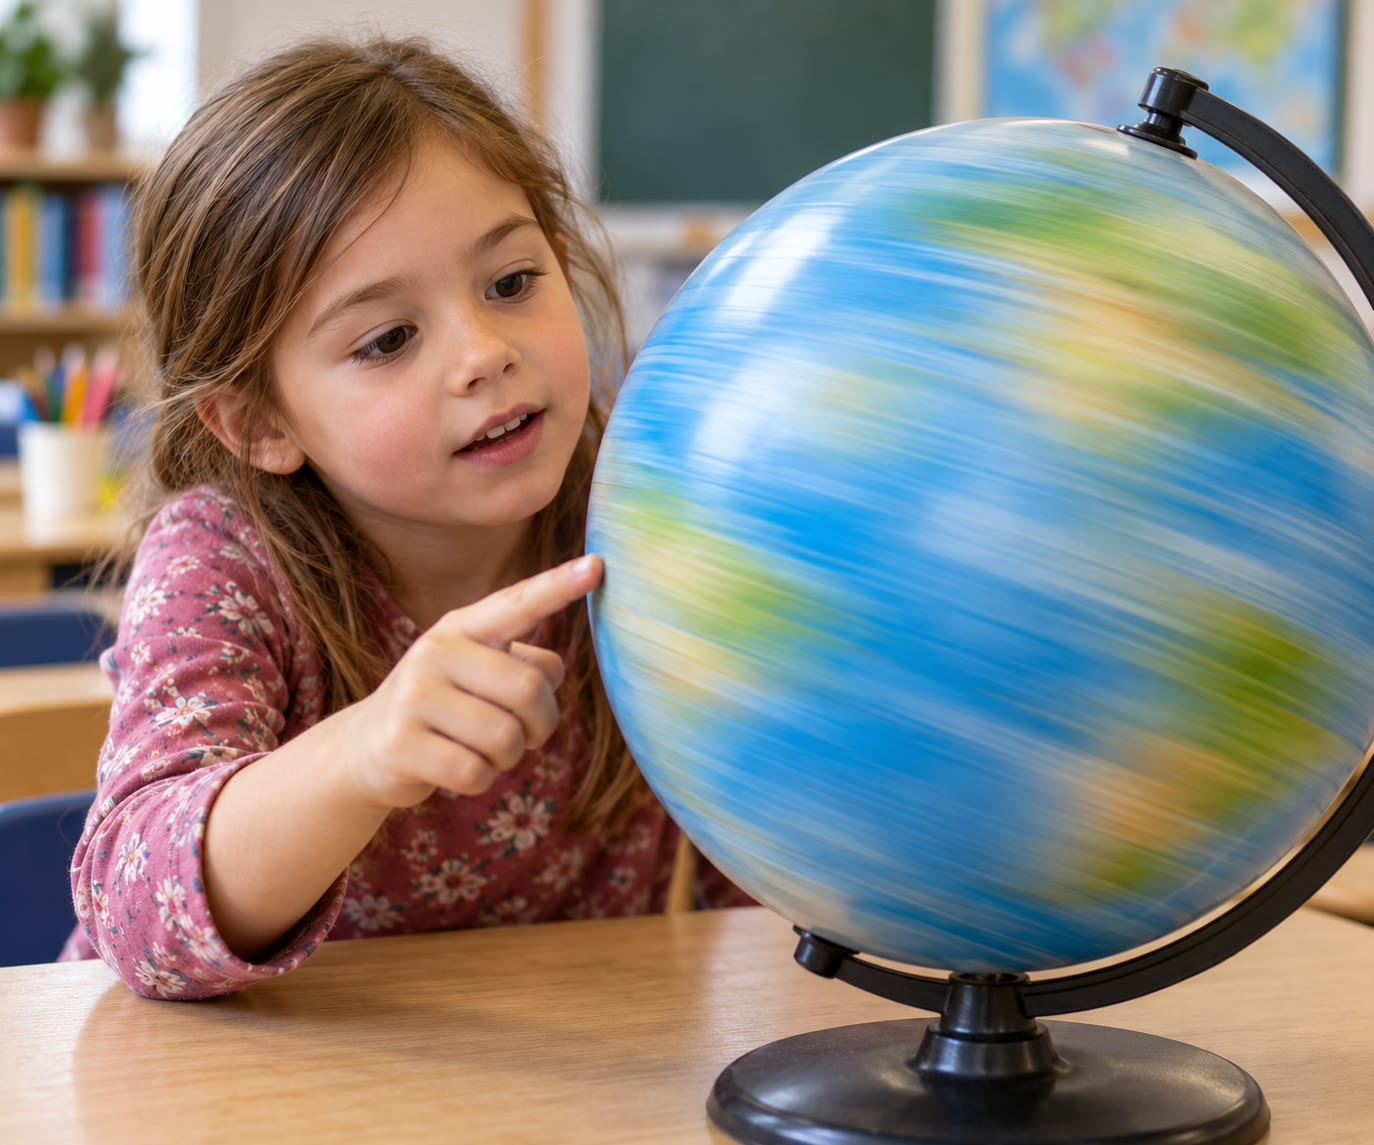
\includegraphics[width=0.6\linewidth]{images/book1/ai/g3-spinning-globe.jpg}

{\small Um \omterm{def:g3:continents-and-oceans:globe}{globo} girando no suporte: a terra e o \omterm{def:g2:water-on-earth:ocean}{mar} passam embaixo do
dedo.}
\end{omfigure}

\begin{recall}
A maior parte da Terra é coberta de \omterm{def:g2:water-on-earth:salt-fresh}{água salgada}: cerca de 71 quadrados em
100 na grade do \cref{ch:g2:water-on-earth}. Um \omterm{def:g2:water-on-earth:ocean}{oceano} é uma extensão
enorme de \omterm{def:g2:water-on-earth:salt-fresh}{água salgada} entre as grandes massas de terra; um \omterm{def:g2:water-on-earth:ocean}{mar} é uma
extensão menor, na beira de um \omterm{def:g2:water-on-earth:ocean}{oceano}. Um \omterm{def:g2:drawing-to-map:map}{mapa} é o desenho de um lugar
visto de cima, feito menor (\cref{ch:g2:drawing-to-map}). Os livros de
física contam como a Terra gira em torno de si mesma uma vez por dia, o
que nos dá o dia e a noite.
\end{recall}

\section{O globo, um pequeno modelo da Terra redonda}

A Terra é redonda, como uma bola muito grande. Não conseguimos ver a sua
forma daqui do chão, porque ela é grande demais: onde quer que estejamos,
o chão parece plano. Mas os astronautas que viajaram para longe da Terra a
viram inteira, uma bola azul e redonda no céu negro (a foto do começo do
\cref{ch:g2:water-on-earth}).

Para ver a Terra inteira numa sala de aula, nós a fazemos pequena.

\begin{definition}[Globo]\label{def:g3:continents-and-oceans:globe}
Um \emph{globo}\index{globo} é um modelo da Terra: uma bola em que a terra
e os \omterm{def:g2:water-on-earth:ocean}{oceanos} estão desenhados com as mesmas formas que na Terra de verdade,
só que muito, muito menores.
\end{definition}

O \omterm{def:g3:continents-and-oceans:globe}{globo} é a melhor imagem da Terra, porque tem a forma certa: redonda. Mas,
como na Terra de verdade, só conseguimos ver uma metade dele de cada vez.
Para ver a outra metade, nós o giramos.

\begin{omfigure}
\begin{tikzpicture}
\begin{axis}[name=atl, hide axis, axis equal image, scale only axis,
    width=6.2cm, xmin=-1.05, xmax=1.05, ymin=-1.05, ymax=1.05, clip=false]
  \fill[omSea] (axis cs:0,0) circle[radius=1];
  \addplot[fill=omHypsLandA!85!black, draw=black!45, line width=0.2pt]
    table {figdata/out/grade-3-globe-atlantic-land.dat};
  \addplot[black!60, dashed, line width=0.5pt]
    table {figdata/out/grade-3-globe-atlantic-equator.dat};
  \addplot[only marks, mark=*, mark size=1.4pt, black]
    table[x=x, y=y] {figdata/out/grade-3-globe-atlantic-poles.dat};
  \addplot[only marks, mark=none, nodes near coords, point meta=explicit symbolic,
    nodes near coords style={font=\scriptsize, anchor=center, fill=white, fill opacity=0.7, text opacity=1, inner sep=1pt, rounded corners=1pt}]
    table[x=x, y=y, meta=name, row sep=\\] {name x y\\ América~do~Norte -0.683 0.636\\ América~do~Sul -0.561 -0.408\\ Europa 0.396 0.639\\ África 0.704 -0.098\\ Oceano~Atlântico -0.209 0.128\\ };
  \draw[black!70, line width=0.8pt] (axis cs:0,0) circle[radius=1];
  \node[font=\scriptsize, anchor=south] at (axis cs:0,0.97) {Polo Norte};
\end{axis}
\begin{axis}[at={(atl.east)}, anchor=west, xshift=0.6cm, hide axis,
    axis equal image, scale only axis,
    width=6.2cm, xmin=-1.05, xmax=1.05, ymin=-1.05, ymax=1.05, clip=false]
  \fill[omSea] (axis cs:0,0) circle[radius=1];
  \addplot[fill=omHypsLandA!85!black, draw=black!45, line width=0.2pt]
    table {figdata/out/grade-3-globe-pacific-land.dat};
  \addplot[black!60, dashed, line width=0.5pt]
    table {figdata/out/grade-3-globe-pacific-equator.dat};
  \addplot[only marks, mark=none, nodes near coords, point meta=explicit symbolic,
    nodes near coords style={font=\scriptsize, anchor=center, fill=white, fill opacity=0.7, text opacity=1, inner sep=1pt, rounded corners=1pt}]
    table[x=x, y=y, meta=name, row sep=\\] {name x y\\ Austrália -0.754 -0.391\\ Oceano~Pacífico 0.258 0.087\\ };
  \draw[black!70, line width=0.8pt] (axis cs:0,0) circle[radius=1];
\end{axis}
\end{tikzpicture}

{\small O \omterm{def:g3:continents-and-oceans:globe}{globo} visto de dois lados. À esquerda: o lado do \omterm{def:g2:water-on-earth:ocean}{oceano} Atlântico,
com as Américas, a Europa e a África. À direita: o outro lado, o \omterm{def:g2:water-on-earth:ocean}{oceano}
Pacífico, com a Austrália na beirada. A linha tracejada é o \omterm{def:g3:continents-and-oceans:equator}{equador}.
Contornos das costas: Natural Earth (domínio público).}
\label{fig:g3:continents-and-oceans:globes}
% ledger: data:ne-land
\end{omfigure}

\begin{remark}[Duas metades muito diferentes]\label{rem:g3:continents-and-oceans:halves}
Observe as duas imagens. À esquerda, a terra cobre cerca de 4 partes da
imagem em 10. À direita, só cerca de 1 parte em 10: o lado do Pacífico é
quase todo de água. Se o dedo de Lena parar desse lado do \omterm{def:g3:continents-and-oceans:globe}{globo}, quase
sempre vai cair no \omterm{def:g2:water-on-earth:ocean}{mar}.
\end{remark}

\section{O equador, os polos e os dois hemisférios}

Um \omterm{def:g3:continents-and-oceans:globe}{globo} gira em torno de uma haste que o atravessa de cima a baixo. A
Terra de verdade não tem haste, mas também gira em torno de uma linha que
passa pelo seu meio. Os dois lugares onde essa linha sai da Terra têm nome.

\begin{definition}[Polo]\label{def:g3:continents-and-oceans:poles}
O \emph{Polo Norte}\index{Polo Norte} e o \emph{Polo
Sul}\index{Polo Sul} são os dois pontos bem no alto e bem embaixo da Terra,
onde sai a linha em torno da qual a Terra gira. Cada um deles é um
\emph{polo}\index{polo}. Num \omterm{def:g3:continents-and-oceans:globe}{globo}, o Polo Norte fica no alto.
\end{definition}

\begin{definition}[Equador e hemisfério]\label{def:g3:continents-and-oceans:equator}
O \emph{equador}\index{equador} é uma linha imaginária traçada em volta de
toda a Terra, exatamente no meio do caminho entre o \omterm{def:g3:continents-and-oceans:poles}{Polo Norte} e o \omterm{def:g3:continents-and-oceans:poles}{Polo Sul}.
Ele divide a Terra em duas metades, e cada uma se chama
\emph{hemisfério}\index{hemisferio@hemisfério}: o \emph{hemisfério
norte}\index{hemisferio norte@hemisfério norte}, do lado do \omterm{def:g3:continents-and-oceans:poles}{Polo Norte}, e
o \emph{hemisfério sul}\index{hemisferio sul@hemisfério sul}, do lado do
\omterm{def:g3:continents-and-oceans:poles}{Polo Sul}.
\end{definition}

O \omterm{def:g3:continents-and-oceans:equator}{equador} não está pintado no chão: ninguém consegue vê-lo numa praia ou
numa floresta. Ele é desenhado nos \omterm{def:g3:continents-and-oceans:globe}{globos} e nos \omterm{def:g2:drawing-to-map:map}{mapas} para nos ajudar a
nos localizar.

\begin{omfigure}
\begin{tikzpicture}[font=\small]
  % globe outline
  \fill[omSea!70] (0,0) circle (2.2);
  % northern hemisphere tinted
  \begin{scope}
    \clip (0,0) circle (2.2);
    \fill[yellow!25, opacity=0.8] (-2.3,0) -- (-2.3,2.3) -- (2.3,2.3) -- (2.3,0)
      arc[start angle=0, end angle=-180, x radius=2.3, y radius=0.45] -- cycle;
  \end{scope}
  \draw[black!70, line width=0.8pt] (0,0) circle (2.2);
  % equator: front half solid, back half dashed
  \draw[red!70!black, line width=1.2pt] (-2.2,0) arc[start angle=180, end angle=360, x radius=2.2, y radius=0.4];
  \draw[red!70!black, line width=0.8pt, dashed] (2.2,0) arc[start angle=0, end angle=180, x radius=2.2, y radius=0.4];
  % axis and poles
  \draw[black!60, line width=0.6pt] (0,2.2) -- (0,2.75);
  \draw[black!60, line width=0.6pt] (0,-2.2) -- (0,-2.75);
  \draw[black!60, line width=0.6pt, dotted] (0,2.2) -- (0,-2.2);
  \fill (0,2.2) circle (2.2pt);
  \fill (0,-2.2) circle (2.2pt);
  \node[anchor=west] at (0.15,2.6) {Polo Norte};
  \node[anchor=west] at (0.15,-2.6) {Polo Sul};
  % labels
  \node[anchor=west] at (2.6,0) {equador};
  \draw[black!60] (2.55,0) -- (2.05,-0.15);
  \node[anchor=west, align=left] at (2.6,1.4) {hemisfério\\norte};
  \draw[black!60] (2.55,1.4) -- (1.5,1.2);
  \node[anchor=west, align=left] at (2.6,-1.4) {hemisfério\\sul};
  \draw[black!60] (2.55,-1.4) -- (1.5,-1.2);
\end{tikzpicture}

{\small O \omterm{def:g3:continents-and-oceans:equator}{equador} divide a Terra em dois \omterm{def:g3:continents-and-oceans:equator}{hemisférios}. O \omterm{def:g3:continents-and-oceans:equator}{hemisfério norte}
(colorido) fica do lado do \omterm{def:g3:continents-and-oceans:poles}{Polo Norte}; o \omterm{def:g3:continents-and-oceans:equator}{hemisfério sul}, do lado do \omterm{def:g3:continents-and-oceans:poles}{Polo Sul}.}
\label{fig:g3:continents-and-oceans:hemispheres}
\end{omfigure}

\begin{example}[Quente perto do equador, frio perto dos polos]\label{ex:g3:continents-and-oceans:hot-cold}
As terras perto do \omterm{def:g3:continents-and-oceans:equator}{equador} são quentes o ano inteiro: é ali que crescem as
grandes florestas tropicais. As terras perto dos \omterm{def:g3:continents-and-oceans:poles}{polos} são frias o ano
inteiro, e grande parte delas é coberta de gelo. Num ano mais adiante você
vai aprender por que é assim; por enquanto, lembre-se: quanto mais perto
de um \omterm{def:g3:continents-and-oceans:poles}{polo}, mais frio.
\end{example}

\section{Sete continentes e cinco oceanos}

Num \omterm{def:g3:continents-and-oceans:globe}{globo}, a terra não está espalhada em pedacinhos por toda parte. A maior
parte dela está reunida em algumas massas muito grandes.

\begin{definition}[Continente]\label{def:g3:continents-and-oceans:continent}
Um \emph{continente}\index{continente} é uma das massas de terra muito
grandes da Terra, junto com as ilhas que ficam perto dela.
\end{definition}

Na maioria das vezes, contamos sete \omterm{def:g3:continents-and-oceans:continent}{continentes}. Do maior para o menor,
eles são: a Ásia, a África, a América do Norte, a América do Sul, a
Antártida, a Europa e a Oceania (a Austrália e as ilhas próximas).
% ledger: natgeo:seven-continents

\begin{center}\small
\begin{tabular}{rlll}
\hline
Tamanho & \omterm{def:g3:continents-and-oceans:continent}{Continente} & \omterm{def:g3:continents-and-oceans:equator}{Hemisfério} & Um detalhe \\
\hline
1 & Ásia & principalmente norte & o maior \\
2 & África & os dois & o \omterm{def:g3:continents-and-oceans:equator}{equador} passa pelo meio \\
3 & América do Norte & norte & vai muito longe para o norte \\
4 & América do Sul & principalmente sul & o \omterm{def:g3:continents-and-oceans:equator}{equador} passa pelo norte \\
5 & Antártida & sul & em volta do \omterm{def:g3:continents-and-oceans:poles}{Polo Sul}, sob o gelo \\
6 & Europa & norte & ligada à Ásia pelo lado leste \\
7 & Oceania & sul & o menor \\
\hline
\end{tabular}
\end{center}

\begin{remark}[Onde termina um continente?]\label{rem:g3:continents-and-oceans:where}
Alguns \omterm{def:g3:continents-and-oceans:continent}{continentes} são cercados de \omterm{def:g2:water-on-earth:ocean}{mar} por todos os lados, como a Oceania
ou a Antártida. Outros se tocam: a Europa e a Ásia formam uma única massa
de terra, e foram as pessoas que escolheram onde traçar a linha entre elas.
É por isso que algumas pessoas contam seis \omterm{def:g3:continents-and-oceans:continent}{continentes}, ou até menos.
\end{remark}

Entre os \omterm{def:g3:continents-and-oceans:continent}{continentes} ficam os \omterm{def:g2:water-on-earth:ocean}{oceanos}. Eles são cinco. O maior é o
\emph{\omterm{def:g2:water-on-earth:ocean}{oceano} Pacífico}; depois vêm o \emph{\omterm{def:g2:water-on-earth:ocean}{oceano} Atlântico}, o
\emph{\omterm{def:g2:water-on-earth:ocean}{oceano} Índico}, o \emph{\omterm{def:g2:water-on-earth:ocean}{oceano} Austral}, em volta da Antártida, e o
menor, o \emph{\omterm{def:g2:water-on-earth:ocean}{oceano} Ártico}, em volta do \omterm{def:g3:continents-and-oceans:poles}{Polo Norte}. Durante muito
tempo, as pessoas contavam só quatro; hoje, a maioria dos países conta o
\omterm{def:g2:water-on-earth:ocean}{oceano} Austral como o quinto.
% ledger: nos:five-oceans, nos:pacific-largest, oer:arctic-smallest

\begin{example}[Qual é o tamanho do Pacífico?]\label{ex:g3:continents-and-oceans:pacific}
O \omterm{def:g2:water-on-earth:ocean}{oceano} Pacífico é tão grande que todos os \omterm{def:g3:continents-and-oceans:continent}{continentes} juntos caberiam
dentro dele. Ele guarda mais da metade de toda a água dos \omterm{def:g2:water-on-earth:ocean}{oceanos} da
Terra. É por isso que o \omterm{def:g3:continents-and-oceans:globe}{globo} da direita, na primeira seção deste
capítulo, parece quase todo azul.
% ledger: nos:pacific-largest
\end{example}

\begin{method}[Dar o nome do oceano entre dois continentes]\label{met:g3:continents-and-oceans:between}
Para descobrir que \omterm{def:g2:water-on-earth:ocean}{oceano} fica entre dois \omterm{def:g3:continents-and-oceans:continent}{continentes}, ponha um dedo em
cada um deles no \omterm{def:g3:continents-and-oceans:globe}{globo} e gire o \omterm{def:g3:continents-and-oceans:globe}{globo} até ver os dois. O \omterm{def:g2:water-on-earth:ocean}{oceano} que o seu
olho atravessa para ir de um dedo ao outro é o que fica entre eles. Num
\omterm{def:g3:continents-and-oceans:globe}{globo}, muitas vezes há dois caminhos possíveis: escolha o mais curto.
\end{method}

\begin{example}[A África e a Austrália]\label{ex:g3:continents-and-oceans:africa-australia}
Indo da África para o leste, em direção à Austrália, atravessamos o \omterm{def:g2:water-on-earth:ocean}{oceano}
Índico. Indo da Europa para o oeste, até a América do Norte, atravessamos
o \omterm{def:g2:water-on-earth:ocean}{oceano} Atlântico. Indo da Ásia para o leste, até a América do Norte,
atravessamos o \omterm{def:g2:water-on-earth:ocean}{oceano} Pacífico.
\end{example}

\section{Um mapa-múndi é um globo achatado}

Um \omterm{def:g3:continents-and-oceans:globe}{globo} é redondo; por isso não é fácil de carregar, e nunca conseguimos
ver ele todo de uma vez. Um \omterm{def:g2:drawing-to-map:map}{mapa} numa folha de papel mostra a Terra inteira
com um só olhar.

\begin{definition}[Mapa-múndi]\label{def:g3:continents-and-oceans:world-map}
Um \emph{mapa-múndi}\index{mapa-mundi@mapa-múndi} é um \omterm{def:g2:drawing-to-map:map}{mapa} da Terra inteira
desenhado plano, numa folha de papel ou numa tela, com todos os
\omterm{def:g3:continents-and-oceans:continent}{continentes} e todos os \omterm{def:g2:water-on-earth:ocean}{oceanos} numa só imagem.
\end{definition}

\begin{omfigure}
\begin{tikzpicture}
\begin{axis}[ommap, width=\linewidth, xtick=\empty, ytick={0},
    yticklabels={equador}, grid=none, clip=true]
  \addplot[fill=omHypsLandA!85!black, draw=black!45, line width=0.2pt]
    table {figdata/out/shared-geo-land.dat};
  \draw[black!60, dashed, line width=0.5pt] (axis cs:-180,0) -- (axis cs:180,0);
  \begin{scope}[every node/.style={font=\scriptsize, align=center}]
    \node at (axis cs:-102,47) {América\\do Norte};
    \node at (axis cs:-60,-12) {América\\do Sul};
    \node at (axis cs:17,52) {Europa};
    \node at (axis cs:20,6) {África};
    \node at (axis cs:92,48) {Ásia};
    \node at (axis cs:134,-24) {Oceania};
    \node at (axis cs:40,-80) {Antártida};
  \end{scope}
  \begin{scope}[every node/.style={font=\scriptsize\itshape, align=center, text=omSea!35!black}]
    \node at (axis cs:-145,8) {Oceano\\Pacífico};
    \node at (axis cs:165,12) {Oceano\\Pacífico};
    \node at (axis cs:-38,22) {Oceano\\Atlântico};
    \node at (axis cs:-15,-25) {Oceano\\Atlântico};
    \node at (axis cs:78,-22) {Oceano\\Índico};
    \node at (axis cs:-115,-57) {Oceano Austral};
    \node at (axis cs:-150,79) {Oceano Ártico};
  \end{scope}
\end{axis}
\end{tikzpicture}

{\small Um \omterm{def:g3:continents-and-oceans:world-map}{mapa-múndi}. O \omterm{def:g3:continents-and-oceans:globe}{globo} foi cortado ao longo de uma linha que passa
pelo meio do \omterm{def:g2:water-on-earth:ocean}{oceano} Pacífico e esticado até ficar plano: o Pacífico aparece
duas vezes, na beirada da esquerda e na da direita. A Antártida, um
\omterm{def:g3:continents-and-oceans:continent}{continente} redondo em volta do \omterm{def:g3:continents-and-oceans:poles}{Polo Sul}, fica esticada numa faixa comprida
embaixo. Contornos das costas: Natural Earth (domínio público).}
\label{fig:g3:continents-and-oceans:world-map}
% ledger: data:ne-land
\end{omfigure}

Mas há uma dificuldade. Tente achatar a casca de uma laranja sobre uma
mesa: ela não fica plana sem rasgar ou esticar. O mesmo acontece com a
superfície do \omterm{def:g3:continents-and-oceans:globe}{globo} quando é desenhada plana. Todo \omterm{def:g3:continents-and-oceans:world-map}{mapa-múndi} rasga o \omterm{def:g3:continents-and-oceans:globe}{globo}
em algum lugar, ou estica certas regiões e espreme outras.

\begin{omfigure}
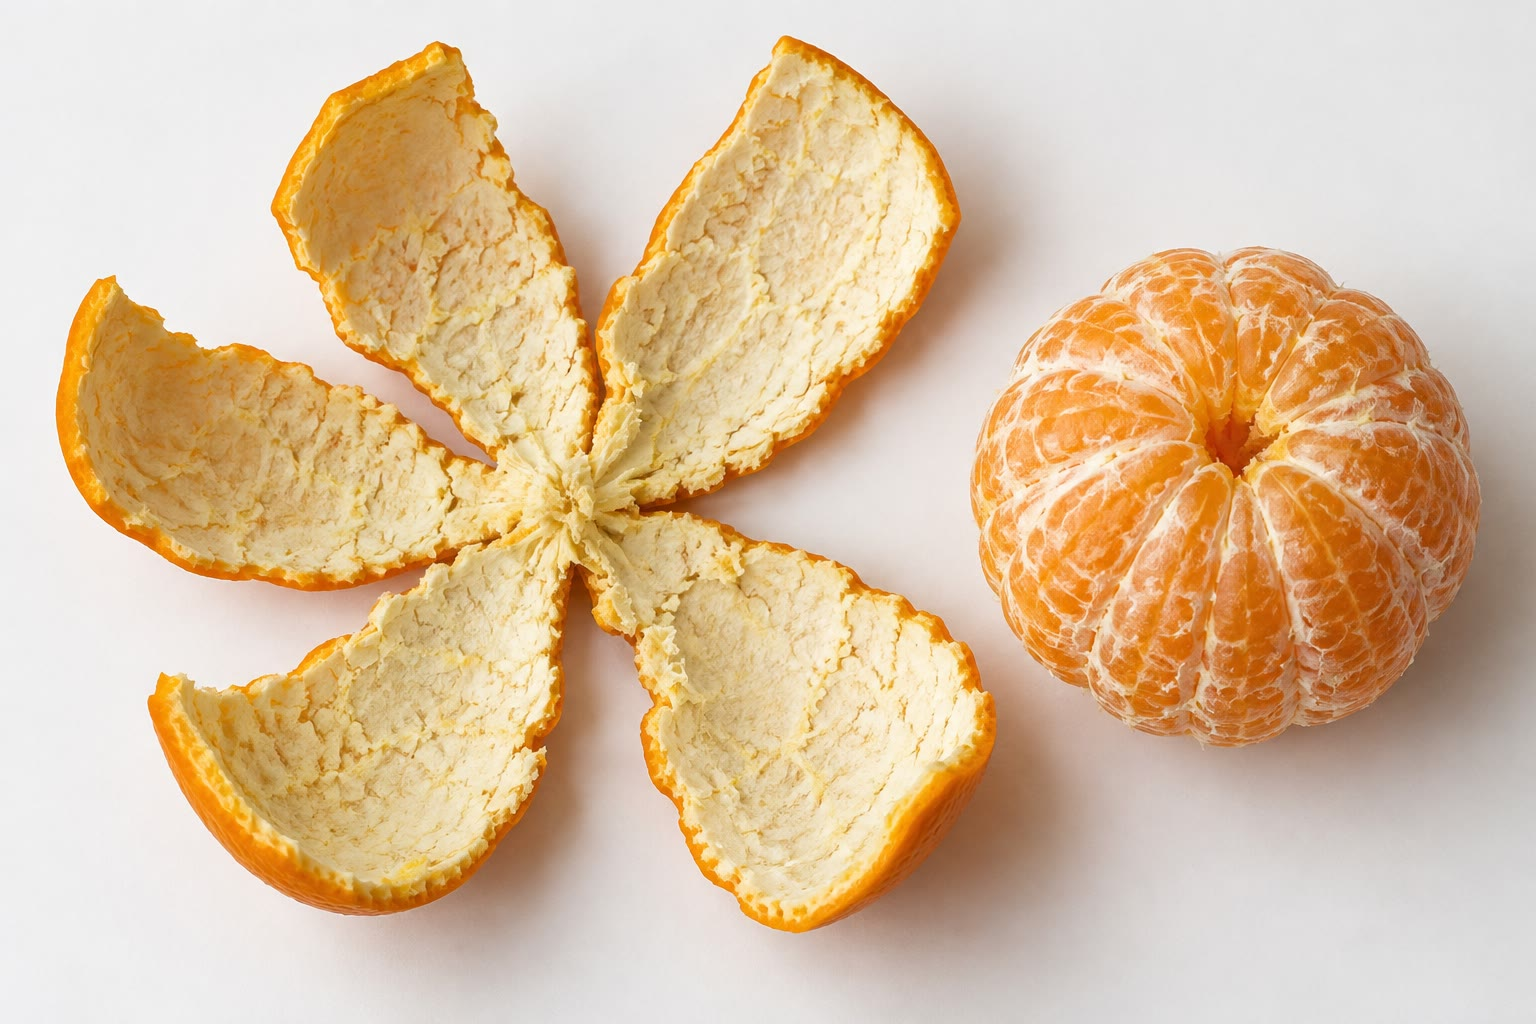
\includegraphics[width=0.4\linewidth]{images/book1/ai/g3-orange-peel.jpg}

{\small A casca de uma laranja não fica plana sem rasgar.}
\end{omfigure}

\begin{remark}[O mapa e o globo não concordam]\label{rem:g3:continents-and-oceans:disagree}
Neste \omterm{def:g3:continents-and-oceans:world-map}{mapa-múndi}, a Antártida parece um dos maiores \omterm{def:g3:continents-and-oceans:continent}{continentes}, esticada
ao longo de toda a beirada de baixo. No \omterm{def:g3:continents-and-oceans:globe}{globo}, ela é uma massa de terra
redonda, menor que a América do Sul. Perto dos \omterm{def:g3:continents-and-oceans:poles}{polos}, um \omterm{def:g2:drawing-to-map:map}{mapa} plano estica
muito a terra. Perto do \omterm{def:g3:continents-and-oceans:equator}{equador}, estica muito pouco. Quando você quiser
comparar o tamanho de dois lugares longe do \omterm{def:g3:continents-and-oceans:equator}{equador}, é o \omterm{def:g3:continents-and-oceans:globe}{globo} que diz a
verdade.
\end{remark}

\begin{method}[Ler um mapa-múndi]\label{met:g3:continents-and-oceans:reading}
Num \omterm{def:g3:continents-and-oceans:world-map}{mapa-múndi} como este:
\begin{enumerate}
  \item o norte fica no alto e o sul embaixo; o \omterm{def:g3:continents-and-oceans:poles}{Polo Norte} é toda a beirada
        de cima, e o \omterm{def:g3:continents-and-oceans:poles}{Polo Sul}, toda a beirada de baixo;
  \item o \omterm{def:g3:continents-and-oceans:equator}{equador} é a linha que atravessa o meio: tudo o que está acima
        dele fica no \omterm{def:g3:continents-and-oceans:equator}{hemisfério norte}, e tudo o que está abaixo, no
        \omterm{def:g3:continents-and-oceans:equator}{hemisfério sul};
  \item a beirada da esquerda e a da direita são a mesma linha no \omterm{def:g3:continents-and-oceans:globe}{globo}: um
        navio que sai pela beirada da direita volta pela da esquerda.
\end{enumerate}
\end{method}

\section{Exercícios}

\begin{exercise}[$\star$]\label{exo:g3:continents-and-oceans:1}
Cite os sete \omterm{def:g3:continents-and-oceans:continent}{continentes}. Qual é o maior? Qual é o menor?
\end{exercise}

\begin{exercise}[$\star$]\label{exo:g3:continents-and-oceans:2}
Cite os cinco \omterm{def:g2:water-on-earth:ocean}{oceanos}. Qual é o maior? Qual é o menor?
\end{exercise}

\begin{exercise}[$\star$]\label{exo:g3:continents-and-oceans:3}
Copie e complete com ``\omterm{def:g3:continents-and-oceans:poles}{Polo Norte}'', ``\omterm{def:g3:continents-and-oceans:poles}{Polo Sul}'' ou ``\omterm{def:g3:continents-and-oceans:equator}{equador}'': o
\dots{} fica no alto de um \omterm{def:g3:continents-and-oceans:globe}{globo}; o \dots{} fica embaixo; o \dots{} dá a
volta inteira pelo meio.
\end{exercise}

\begin{exercise}[$\star$]\label{exo:g3:continents-and-oceans:4}
\omterm{def:g3:continents-and-oceans:equator}{Hemisfério norte} ou \omterm{def:g3:continents-and-oceans:equator}{hemisfério sul}? A Europa; a Oceania; a Antártida; a
América do Norte.
\end{exercise}

\begin{exercise}[$\star$]\label{exo:g3:continents-and-oceans:5}
Que \omterm{def:g2:water-on-earth:ocean}{oceano} fica em volta do \omterm{def:g3:continents-and-oceans:poles}{Polo Norte}? Que \omterm{def:g2:water-on-earth:ocean}{oceano} fica em volta da
Antártida?
\end{exercise}

\begin{exercise}[$\star\star$]\label{exo:g3:continents-and-oceans:6}
Que \omterm{def:g2:water-on-earth:ocean}{oceano} você atravessa para ir da África à América do Sul? E da
Austrália à América do Sul, indo para o leste? E da África à Austrália?
\end{exercise}

\begin{exercise}[$\star\star$]\label{exo:g3:continents-and-oceans:7}
Sam mora num país onde faz calor o ano inteiro. Bo mora numa estação de
pesquisa onde faz um frio de congelar o ano inteiro. Um deles mora perto
do \omterm{def:g3:continents-and-oceans:equator}{equador}, e o outro perto de um \omterm{def:g3:continents-and-oceans:poles}{polo}. Quem mora onde?
\end{exercise}

\begin{exercise}[$\star\star$]\label{exo:g3:continents-and-oceans:8}
Lena gira o \omterm{def:g3:continents-and-oceans:globe}{globo} 10 vezes. O dedo dela cai no \omterm{def:g2:water-on-earth:ocean}{mar} 7 vezes. Quantas vezes
ele cai na terra? É o que você esperava? Por quê?
\end{exercise}

\begin{exercise}[$\star\star$]\label{exo:g3:continents-and-oceans:9}
No \omterm{def:g3:continents-and-oceans:world-map}{mapa-múndi} da página~\pageref{fig:g3:continents-and-oceans:world-map}, o
\omterm{def:g2:water-on-earth:ocean}{oceano} Pacífico aparece duas vezes. Por quê? A Terra de verdade tem dois
\omterm{def:g2:water-on-earth:ocean}{oceanos} Pacíficos?
\end{exercise}

\begin{exercise}[$\star\star\star$]\label{exo:g3:continents-and-oceans:10}
Tom diz: ``No \omterm{def:g3:continents-and-oceans:world-map}{mapa-múndi}, a Antártida é mais comprida que a Ásia; então a
Antártida é o maior \omterm{def:g3:continents-and-oceans:continent}{continente}.'' Tom tem razão? Use a lista dos
\omterm{def:g3:continents-and-oceans:continent}{continentes} do maior para o menor e diga por que o \omterm{def:g3:continents-and-oceans:world-map}{mapa-múndi} o engana.
\end{exercise}
